\documentclass[t]{beamer}

%bibliography
%\usepackage[notes,backend=bibtex,isbn=false,doi=false,eprint=false, note=false, url=false]{biblatex-chicago}
\usepackage[authordate-trad,backend=biber,isbn=false,doi=false,eprint=false, url=true]{biblatex-chicago}
\bibliography{narrative}

\definecolor{links}{HTML}{2A1B81}
\hypersetup{colorlinks,linkcolor=gray,urlcolor=links}

% customizing the title page
\defbeamertemplate*{title page}{customized}[1][]
{
  \vspace{1cm}
  \usebeamerfont{title}\inserttitle\par
  \usebeamerfont{subtitle}\usebeamercolor[fg]{subtitle}\insertsubtitle\par
  \vspace{4.5cm}
  \usebeamerfont{date}\insertdate\par
  \vspace{.5cm}
  \usebeamerfont{author}\insertauthor\par
  \usebeamerfont{institute}\insertinstitute\par
  
  
  \usebeamercolor[fg]{titlegraphic}\inserttitlegraphic
}

\usepackage{graphicx}
\usetheme[compress]{Dresden}
\usecolortheme{dove}
\usefonttheme{serif}
%\usefonttheme{structureitalicserif}
%\usepackage{helvet}
%\usefonttheme{professionalfonts}
%gets rid of bottom navigation bars
\setbeamertemplate{footline}[frame number]{}
\usepackage[utf8]{inputenc}
\usepackage[norsk]{babel}
\usepackage{appendix}
\usepackage[export]{adjustbox}
\usepackage{wrapfig}
\setbeamertemplate{caption}{\insertcaption}
\usepackage{tikz}
\usepackage{multirow} % to have tables with rows over multiple lines
\usepackage{hyperref}

\title{\huge Word emebedding and other frontiers in text analysis}
%\subtitle{What? How? (and a little bit why?)}
%\vspace{6cm} % this doesn't seem to do anything...
\author{Gregory Ferguson-Cradler}
\institute{Institutt for rettsvitenskap, filosofi og internasjonale studier \\ Høgskolen i Innlandet, Lillehammer}
\date{NTNU, Trondheim, 12.-13. August 2021} %\today}
 
% \AtBeginSubsection[]
% {
% \begin{frame}<beamer>{Overview}
% \tableofcontents[currentsection, currentsubsection, currentsubsubsection,
%     %hideothersubsections, 
%     sectionstyle=show/shaded,
% ]
% \end{frame}
% }
 
\begin{document}

\begin{frame}[plain]
    \titlepage    
\end{frame}

% \begin{frame}[plain]%{1944}
% %\frametitle{\vspace{-.5cm}Frame Title Goes Here}
% \begin{figure}
% %\vspace*{-.5cm}
% \includegraphics[width=1\textwidth, valign=c]{Frontene.jpg} 
% %\caption{Frontene i Europa i 1944}
% \end{figure}
% \end{frame}

\section{Word embedding}
\begin{frame}{Word similarity and relatedness}
\begin{enumerate}
    \item Based on the ideas that similar words appear in the same context (both words that are synonyms and words that are simply clearly of the same kind, eg. "Germany" and "France"\footnote{This is based on long and deep thought in linguistics, see \autocite{jurafsky2014speech} for a brief overview}.
    \item Based on the idea that word meaning can be represented in vector space (as we saw in document similarity) based on contexts in which words appear.
    \item Documents made into vectors via DTM matrix. Words might be made into vectors via term-term matrix (fcm in Quanteda)
    \item Two major algorithms for word embedding: word2vec and GloVe. 
\end{enumerate}
\end{frame}

\begin{frame}{What \textit{are} word embeddings}
\begin{itemize}
    \item Simplifying: these algorithms compute probability for word co-occurences (and non-co-occurrences) and construct word embeddings (vectors) that are similar when co-occurence probability is high and distant when probability is low.\footnote{\textcite{jurafsky2014speech} is the best introduction to the details.}
    \item Word embeddings so interesting (and somewhat baffling) because they show not just similarities between words but also have vector spaces that seem to correspond to meaningful concepts. 
    \item $\overrightarrow{king} + \overrightarrow{woman} - \overrightarrow{man} \approx \overrightarrow{queen}$ analagous to just as a human would generally suggest `queen' in answer to the question: man:woman as king:\underline{\hspace{1cm}}?. 
\end{itemize}
\end{frame}

\begin{frame}{Document similarity methods in practice, I}
\begin{itemize}
%\setlength{\itemindent}{1cm}
    \item \fullcite[]{kozlowski2019geometry}
    \item Insight: we find dimensions in vector space that map to human meanings (eg, affluence, etc) by taking the average of pairs of words whose meanings diverge on this range (for affluence: affluence-poverty; rich-poor, prosperous-bankrupt, etc).
    \item Other words can then be "projected" along this dimension to measure where they stand on the spectrum.
\end{itemize}
  \end{frame}

\begin{frame}{Kozlowski et al. 2019}
\vspace*{\fill}
\begin{figure}
    \centering
    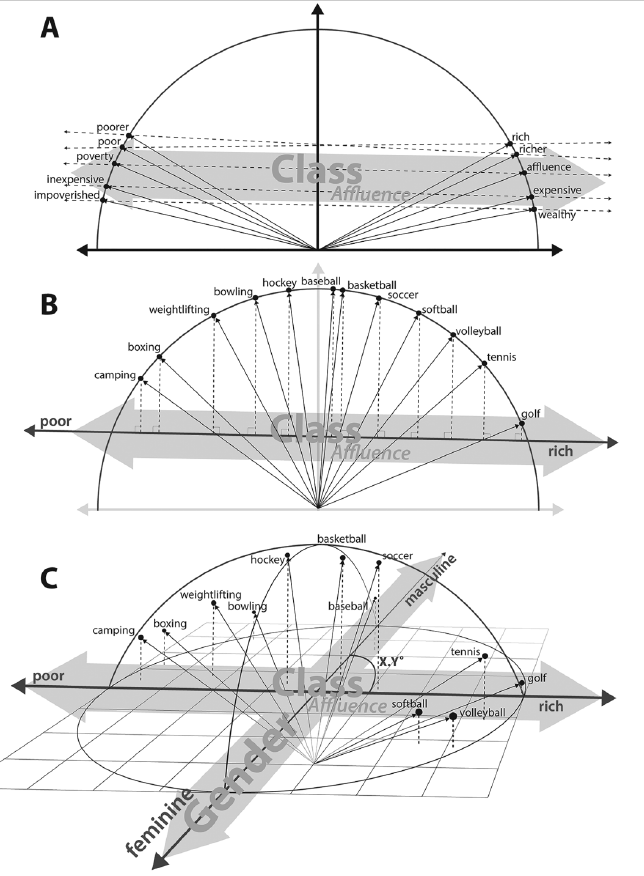
\includegraphics[width = .45\linewidth]{kozlowsik.png}
    \caption{\fullcite[913]{kozlowski2019geometry}}
    \label{fig:my_label}
\end{figure}
\vspace*{\fill}
\end{frame}

\begin{frame}{Document similarity methods in practice, II}
\begin{tabular}{ll}
\adjincludegraphics[width=.5\linewidth]{employer.jpg}
&
 \vspace*{\fill}
\adjincludegraphics[width = .5\textwidth]{culted_reg.jpg}
 \vspace*{\fill}
\end{tabular}
 \autocite[928,924]{kozlowski2019geometry}
 \end{frame}

\section{Frontier methods}
\begin{frame}{Contextualized word emebeddings and transformers}
\begin{itemize}
    \item Individual \textit{token} embeddings
    \item Transformers weigh context word affect words of interest
    \item So far main use in social science seen for classification
    \item Unclear how might be taken up for interpretive purposes
\end{itemize}

\end{frame}


\section{Conclusion}
\begin{frame}{Further resources: textbooks on R and text analysis}
    \begin{itemize}
        \item \fullcite{wickham2016r}
        \item \fullcite{silge2017text}
        \item \fullcite{jurafsky2014speech}
        \item \fullcite{jockers2020text}
    \end{itemize}
\end{frame}

\begin{frame}{Further resources: online courses in programming and R}
\begin{itemize}
    \item \hyperlink{https://www.edx.org/course/introduction-to-computer-science-and-programming}{Introduction to Computer Science and Programming}: solid introduction to basics of programming (in Python but easily applicable to R)
    \item \hyperlink{https://www.edx.org/course/data-analysis-for-social-scientists}{Data analysis for social scientists}: basic quantitative methods in social science in R.
    \item \hyperlink{https://www.edx.org/professional-certificate/harvardx-data-science}{Intro to Data Science}: very basic course in R and data science.
\end{itemize}
\end{frame}

\begin{frame}{Further resources: people in digital humanities/social science to follow}
    \begin{itemize}
        \item \hyperlink{https://benschmidt.org/}{Ben Schmidt}
        \item \hyperlink{https://tedunderwood.com/}{Ted Underwood}
        \item \hyperlink{https://juliasilge.com/}{Julia Silge}
        \item \hyperlink{http://varianceexplained.org/}{David Robinson}
        \item \hyperlink{https://kenbenoit.net/}{Ken Benoit}
    \end{itemize}
\end{frame}

\end{document}

